\documentclass{beamer}

\usepackage{math214}

\usepackage{hyperref}
\usepackage{caption}
\DeclareCaptionLabelFormat{black}{\textcolor{black}{#1~#2}}
\captionsetup[figure]{labelformat=black}
\captionsetup[figure]{font=tiny}
\usepackage{listings}
\usepackage[linesnumbered,ruled]{algorithm2e}


\title{Presentation Topic}
\author{Team member names}
\date{Spring 2023}

\definecolor{darkblue}{HTML}{6666dd} 
%\colortheme{green!42!black}
%\colortheme{orange!85!black}
%\colortheme{darkblue}
%\colortheme{pink!80!black}
%\colortheme{orange!85!white!90!black}

\begin{document}

\maketitle

\section{First section}

\section{Application of Gradient Descent: MNIST}
\begin{frame}{Application Introduction}
	\begin{columns}[T,onlytextwidth]
		\column{.4\textwidth}
		\begin{figure}
			\centering 
			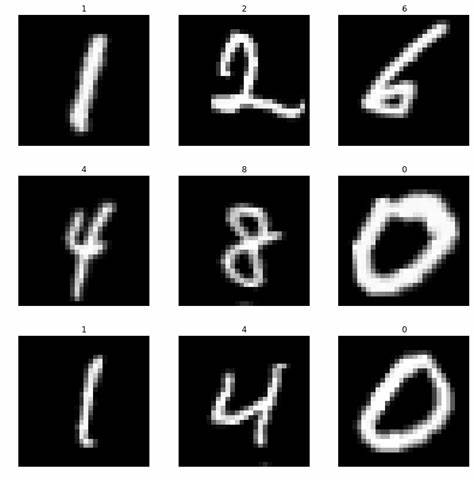
\includegraphics[width=1\columnwidth,height=6cm]{img/mnist.jpg}
			\caption{}
		\end{figure}
	
		\column{.6\textwidth}
		\begin{itemize}
			\item MNIST is a famous dataset used for image
			recognition and classification tasks. It consists 
			of 70,000 (60,000 training+10,000 testing) 
			handwritten digits in a 28x28 px grayscale image.
			\item Our project application is to use CNN model
			predict MNIST handwritten digits. In the application,
			we discover how Gradient Descent applies in DL.
			\item Project source code repo: \href{https://github.com/openhe-hub/math214-project.git}{https://github.com/openhe-hub/math214-project.git} 
		\end{itemize}
	\end{columns}	
\end{frame}

\begin{frame}{Model Introduction}
	\begin{columns}[T,onlytextwidth]
		\column{.4\textwidth}
		\begin{figure}
			\centering 
			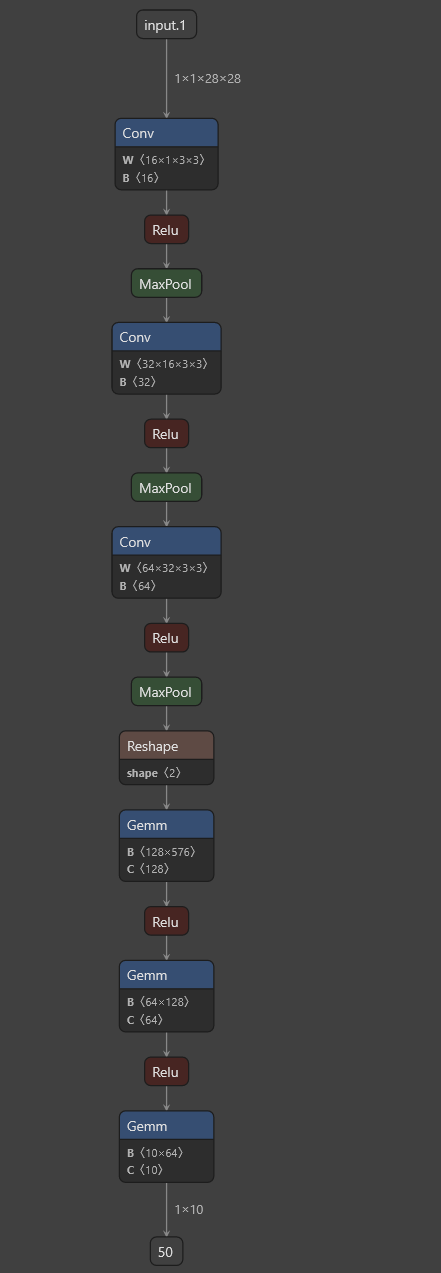
\includegraphics[width=0.85\columnwidth, height=7.5cm]{img/model.png}
			\caption{CNN Model (visualized by Netron)}
		\end{figure}

		\column{.6\textwidth}
		\begin{itemize}
			\item Our CNN Model: \newline 3 $conv\_layers$ (Conv+Relu+MaxPool)\newline+1 $fc\_layer$ (Linear+Relu)
			\item Loss function: $CrossEntropy$
			\item Gradient Descent: $SGD$
			\item Other Parameters: 
				\begin{itemize}
					\item $epochs=30$
					\item $batch\_size=64$
					\item $learning\_rate=0.001$
				\end{itemize}
		\end{itemize}
	\end{columns}
\end{frame}


\begin{frame}{Gradient Descent}
	\begin{theorem}
		SGD Iteration Formula: $w_{t+1} = w_t - \eta \nabla L(w_t)$
	\end{theorem}
	\begin{algorithm}[H]
		\SetAlgoLined
		\KwData{Input data $x$ and labels $y$}
		\KwResult{Trained CNN model}
		\SetKwFunction{FMain}{Train}
		\SetKwProg{Fn}{Function}{:}{}
		\Fn{\FMain{}}{
			\For{$epoch$ =1 to $epochs$}{
				\For{$batch\_i=(x_i,y_i)$ in $dataset$}{
					Set gradients of network parameters to zero\;
					Forward propagation: $\hat{y}$=forward($x_i$)\;
					Compute loss function: $loss$=$L(\hat{y}, y_i)$\;
					Backward propagation: $loss$.backward()\;
					Update parameters using SGD: $w = w - \eta \nabla L(w)$\;
				}
			}
		}
		\caption{SGD algorithm for training a CNN}
	\end{algorithm}
\end{frame}

\begin{frame}{Conclusion}
	\begin{columns}[T,onlytextwidth]
		\column{.45\textwidth}
		\begin{figure}
			\centering 
			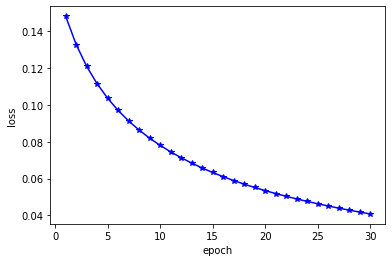
\includegraphics[width=1\columnwidth,height=4.2cm]{img/loss.png}
			\caption{SGD epoch-loss plot}
		\end{figure}

		\column{.05\textwidth}
	
		\column{.5\textwidth}
		  \quad The epoch-loss plot  shows how the model's 
		  loss function changes over time, as it updates the model 
		  parameters using small batches of training data. The plot 
		  typically displays a downward trend, with rapid 
		  loss reductions in initial epochs, and slower reductions 
		  as the algorithm converges. 
	\end{columns}
\end{frame}

\begin{frame}{Classification Result}
	\begin{columns}[T,onlytextwidth]
		\column{.45\textwidth}
		\begin{figure}
			\centering 
			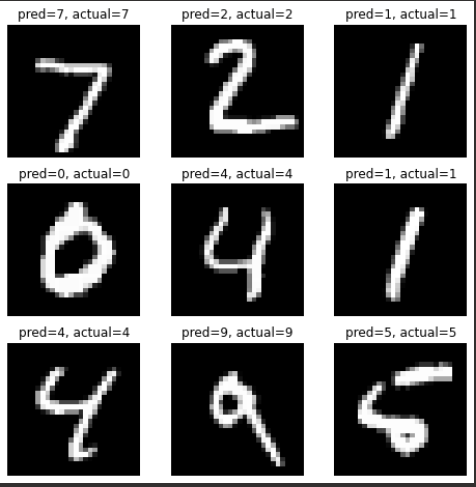
\includegraphics[width=1\columnwidth,height=5.5cm]{img/result.png}
			\caption{Testing set prediction result}
		\end{figure}

		\column{.05\textwidth}
	
		\column{.5\textwidth}
		\begin{itemize}
			\item Result: The total loss is about $0.0413$, 
			and the accuracy is about $98.67\%$. Algorithms (SGD) 
			based on Gradient Descent works well in our CNN model.
			\item Improvement: Consider adjusting
			parameters like $learning\_rate$, $batch\_size$. Also, we may 
			change different GD algorithms like $Adam$.
		\end{itemize} 
	\end{columns}
\end{frame}



\section{Third section}

\section{Fourth section}


\thankframe

\end{document}
